\documentclass[border=4pt]{standalone}
\usepackage{amsmath}
\usepackage{tikz}
\usetikzlibrary{arrows.meta,decorations.pathreplacing}
\definecolor{boxblue}{RGB}{225,238,252}
\definecolor{boxorange}{RGB}{253,236,216}
\definecolor{boxgray}{RGB}{237,237,237}
\begin{document}
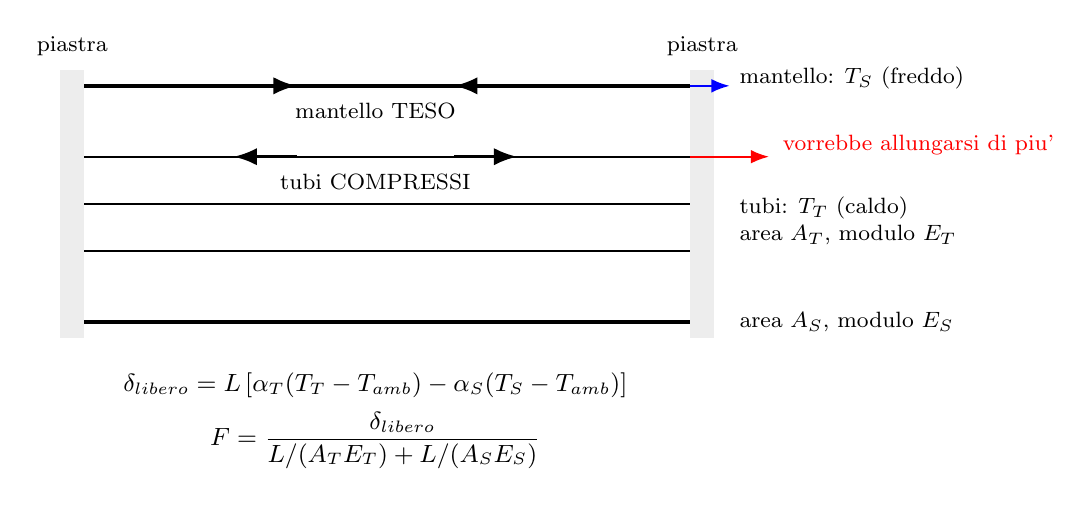
\begin{tikzpicture}[scale=1.0]
% tubesheets
\fill[boxgray] (0,-1.7) rectangle (0.3,1.7);
\fill[boxgray] (8.0,-1.7) rectangle (8.3,1.7);
\node[font=\footnotesize] at (0.15,2.0) {piastra};
\node[font=\footnotesize] at (8.15,2.0) {piastra};
% shell
\draw[very thick] (0.3,1.5) -- (8.0,1.5);
\draw[very thick] (0.3,-1.5) -- (8.0,-1.5);
\node[font=\footnotesize,anchor=west] at (8.5,1.6) {mantello: $T_S$ (freddo)};
\node[font=\footnotesize,anchor=west] at (8.5,-1.5) {area $A_S$, modulo $E_S$};
% tubes
\foreach \y in {-0.6,0,0.6}{ \draw[thick] (0.3,\y) -- (8.0,\y); }
\node[font=\footnotesize,anchor=west] at (8.5,-0.05) {tubi: $T_T$ (caldo)};
\node[font=\footnotesize,anchor=west] at (8.5,-0.4) {area $A_T$, modulo $E_T$};
% free expansion indication
\draw[-{Latex},thick,red] (8.0,0.6) -- (9.0,0.6);
\node[font=\footnotesize,red,anchor=west] at (9.05,0.75) {vorrebbe allungarsi di piu'};
\draw[-{Latex},thick,blue] (8.0,1.5) -- (8.5,1.5);
% force arrows
\draw[-{Latex},very thick] (3.0,0.6) -- (2.2,0.6);
\draw[-{Latex},very thick] (5.0,0.6) -- (5.8,0.6);
\node[font=\footnotesize] at (4.0,0.28) {tubi COMPRESSI};
\draw[-{Latex},very thick] (2.2,1.5) -- (3.0,1.5);
\draw[-{Latex},very thick] (5.8,1.5) -- (5.0,1.5);
\node[font=\footnotesize] at (4.0,1.18) {mantello TESO};
\node[font=\small] at (4.0,-2.3) {$\delta_{libero}=L\left[\alpha_T(T_T-T_{amb})-\alpha_S(T_S-T_{amb})\right]$};
\node[font=\small] at (4.0,-3.0) {$F=\dfrac{\delta_{libero}}{L/(A_T E_T)+L/(A_S E_S)}$};
\end{tikzpicture}
\end{document}
